\chapter{Results} % Main chapter title

\label{chap:results} % For referencing the chapter elsewhere, use \ref{Chapter1} 

\section{Semantic Embeddings}
\subsection{Validation on English Data}
For \code{SIM} space, we used the English \code{WordNetEmbedding} trained on the first 15,000 frequent words and benchmark dataset vocabulary. We kept first 511 PCs by following the method in Section \ref{subsec:semanticsimilaritymethod}, which is comparable to the best dimensionality (850) reported by the original work \parencite{saediWordNetEmbeddings2018} for a \code{WordNetEmbedding} keeping all semantic relations.

The intersection of \code{SIM} space and the Common Crawl vocabulary used in \code{MIX} space resulted to 8157 words. 

The linear regression model mapping \code{SIM} to \code{MIX} produced a \code{r2} score of 0.1662.

Figure \ref{fig:EngDecorVarRatio} shows the PCA-factored explained variances of the 4 resulting semantic space PCs. Table \ref{tab:engdecorrelationscores} shows the semantic ranking task evaluations. Conformably to our hypotheses, the untouched \code{MIX} space is indeed a mixture of \similarity and \association information. \code{SIM}, which is constructed with specifically picked semantic relations from \code{WordNet}, is purely \similarity with statistically negligible \association scores. Though we have not completely purged \similarity information from \code{ASN} and \association from \code{SIG}, each resulting semantic space has significantly reduced the score in its irrelevant semantic axis. In addition, a clear dominance of \association semantic signal is present in \code{ASN} and \similarity in \code{SIG}. 


\begin{figure}
    \centering
    \makebox[\linewidth]{
    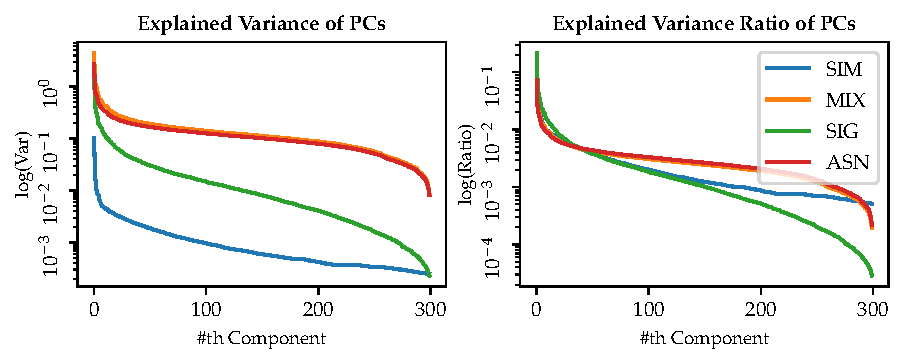
\includegraphics[scale=.8]{Figures/EngDecorVarRatio.pdf}
    }
    \caption[EVR of 4 Semantic Spaces, English]{PCA of 4 semantic spaces of the English 8157 vocabulary. \textbf{Left panel}: While the variance of \code{SIM} is systematically smaller than other three spaces, its projection (\code{SIG}) has larger variances. The suppression of \code{SIG} from \code{MIX} has little impact on \code{MIX}'s variance. \textbf{Right panel}: \code{SIG} and \code{SIM} have a denser variance concentrated on first PCs, while \code{ASN} and \code{MIX} have more homogeneous variance distributions.} 
    \label{fig:EngDecorVarRatio}
\end{figure}

\begin{table}
    \centering
    \begin{ThreePartTable}
        
    \begin{tabularx}{\textwidth}{RRRRll}
        \multicolumn{6}{l}{\tabhead{English Semantic Space Semantic Ranking Task Results}} \\
    \toprule
    \tabhead{Semantic Space} & \tabhead{Vocabulary Size} & \tabhead{Dimension} & r & \tabhead{SimLex-999} & \tabhead{WS353-ASN} \\  
    \midrule
    \mr{2}{*}{\code{SIM}} & \mr{2}{*}{15K} & \mr{2}{*}{511} & Pearson & .5060 & \textbf{.0279}\tnote{1} \\  
    &  &  & Spearman & .4989 & \textbf{.0193}\tnote{2}   \\  
    \midrule
    \mr{2}{*}{\code{MIX}} & \mr{2}{*}{2.2M} & \mr{2}{*}{300} & Pearson & .3946 & .6091 \\  
    &  &  & Spearman & .3752 & .5709 \\  
    \midrule
    \mr{2}{*}{\code{ASN}} & \mr{4}{*}{8157} & \mr{4}{*}{300} & Pearson & .1953 & .5633 \\  
    &  &  & Spearman & .2133 & .5918 \\ 
    
    \cmidrule{1-1} \cmidrule{4-6}
    \mr{2}{*}{\code{SIG}} &  &  & Pearson & .4929 & .2091 \\  
    &  &  & Spearman & .4994 & .1678 \\  
    
    \cmidrule{2-6}
    \multicolumn{4}{r}{Out of Vocabulary} & .002 & .024 \\  
    \midrule \midrule
    \mr{2}{*}{Baseline\tnote{3}} & \mr{2}{*}{13k} & \mr{2}{*}{850} & Pearson & .50 & .32 \\  
        &  &  & Spearman & .52 & .33 \\  
    \bottomrule
    \end{tabularx}
    \begin{tablenotes}
        \footnotesize
        \item Scores marked in bold have a p-value larger than 0.05.
        \item[1] p-value=0.6626
        \item[2] p-value=0.7629
        \item[3] Baseline is reported by \textcite{saediWordNetEmbeddings2018}. The 13k words are selected cue words in psycholinguistic experiments. They show the best performance among all tested models.
    \end{tablenotes}
    \end{ThreePartTable}
    \caption[English Semantic Space Semantic Ranking Task Results]{With a different semantic relation selection, \code{SIM} achieves almost the same performance as the baseline in \similarity benchmark, while it cancels out the 
    \association score. \code{MIX} space performs well in both task-sets, with a slight preference for \association, consistent with \parencite{lapesaContrastingSyntagmaticParadigmatic2014}'s conclusion. \code{ASN} has comparable scores in \association with \code{MIX}, but still have a non-zero score in \similarity. The projected \code{SIG} space compared with \code{SIM} has similar scores in \similarity and a much lower score in \association.\label{tab:engdecorrelationscores}}
    \end{table}

\subsection{Application on French data}

Provided with the methodological success of English data, we applied the same algorithm against French data.

For \code{SIM} space, we used the French \code{WOLFEmbedding} with POS tag trained on all the available vocabulary. We kept first 634 PCs.

After rule-based and manual matching, the intersection of \code{SIM} space and the \code{MIX} space vocabulary resulted to 24519 distinct lemma with POS tags.

The linear regression model mapping \code{SIM} to \code{MIX} produced a \code{r2} score of 0.0776, which is lower than the English score, indicating a smaller informational overlap between the two embedding models.

Figure \ref{fig:FreDecorVarRatio} shows a similar PCA explained variance distribution. Though no sound evidence supporting the validity of the French benchmarks, we tested the resulting semantic spaces using the same tasks against our indicative gold-standard data (Section \ref{subsection:frenchbenchmarkdataconstruction}). The unmodified \code{MIX} space has a much lower score in \similarity and \association compared to the English \code{MIX}, setting a weak baseline for embedding space comparison. Again, \code{SIM} achieves high scores in \similarity, and negligible scores in \association. However, the results (Table \ref{tab:fredecorrelationscores}) puts the validity of \code{ASN} space into question: viewed by Pearson's \code{r} it seems to contain none of \similarity and \association information, judged by Spearman's \code{r}, both axes' information are present in the space. All p-values reported for \code{ASN} are close to the significance threshold. However, \association scores of \code{ASN} are nevertheless higher than \similarity scores. Despite that \code{SIG} represents only a very small portion of variances of the \code{MIX} embedding as indicated by a low \code{r2} score, \code{SIG} has comparable \similarity scores as \code{SIM}, and the purity against \association is even more remarked. 

\begin{figure}
    \centering
    \makebox[\linewidth]{
    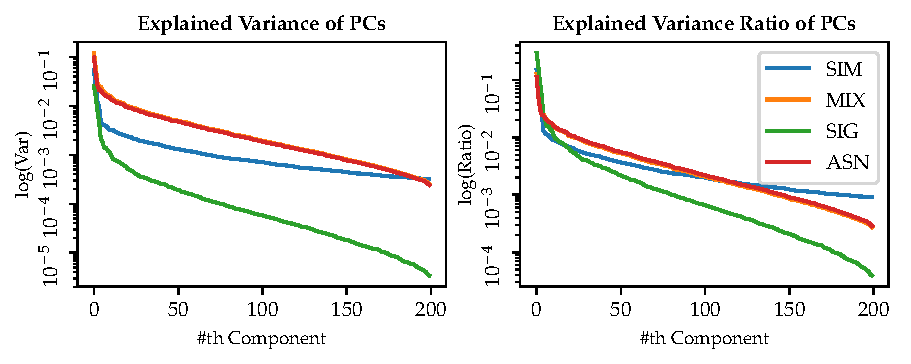
\includegraphics[scale=0.8]{Figures/FreDecorVarRatio.pdf}
    }
    \caption[EVR of 4 Semantic Spaces, French]{PCA of 4 semantic spaces of the French 24519 vocabulary. \textbf{Left panel}: Due to the poor linear correlation found between \code{SIM} and \code{MIX}, the variance of \code{SIG} is systematically smaller than the other three spaces, the original space \code{SIM} has larger variances. The suppression of \code{SIG} from \code{MIX} has also little impact on the model's variance. \textbf{Right panel}: \code{SIG} has a denser variance concentrated on first PCs, while the other three spaces have more homogeneous variance distributions.\label{fig:FreDecorVarRatio}} 
    
\end{figure}

\begin{table}
    \centering
    \begin{ThreePartTable}
    
    \begin{tabularx}{\textwidth}{RRRR *{2}{A{2.3cm}}}
        \multicolumn{6}{l}{\tabhead{French Semantic Space Semantic Ranking Task Results}} \\
    \toprule
    \tabhead{Semantic Space} & \tabhead{Vocabulary Size} & \tabhead{Dimension} & r & \tabhead{\emph{Similarity} SimLex-999} & \tabhead{\emph{Association} WS353-ASN} \\  
    \midrule
    
    \mr{5}{*}{\code{SIM}} & \mr{4}{*}{56665} & \mr{4}{*}{634} & Pearson & .3291 & \textbf{.1039} \\  
    &  &  & p-value & 0 & .1061 \\  
    \cmidrule{4-6}
    &  &  & Spearman & .2812 & \textbf{.0511} \\  
    &  &  & p-value & 0 & .4273 \\  
    \cmidrule{2-6}

    \multicolumn{4}{r}{Out of Vocabulary} & .048 & .04 \\  
   \midrule

   \mr{4}{*}{\code{MIX}} & \mr{14}{*}{24519} & \mr{14}{*}{200} & Pearson & .0940 & .1520 \\  
   &  &  & p-value & .0047 & .0197 \\  
   \cmidrule{4-6}

    &  &  & Spearman & .1449 & .2078 \\ 
    &  &  & p-value & 0 & .0014 \\  

    \cmidrule{1-1} \cmidrule{4-6}

   \mr{4}{*}{\code{ASN}} &  &  & Pearson & \textbf{.0629} & \textbf{.1116} \\  
   &  &  & p-value & .0590 & .0879 \\  
   \cmidrule{4-6} 
    &  &  & Spearman & .0771 & .1566 \\  
    &  &  & p-value & .0206 & .0162 \\  

\cmidrule{1-1} \cmidrule{4-6}

   \mr{4}{*}{\code{SIG}} &  &  & Pearson & .2541 & \textbf{-.0044} \\  
   &  &  & p-value & 0 & .9458 \\  
   \cmidrule{4-6}

    &  &  & Spearman & .3121 & \textbf{-.0078} \\  
   &  &  & p-value & 0 & .9050 \\  

    \cmidrule{2-6}

    \multicolumn{4}{r}{Out of Vocabulary} & .0797 & .0711 \\  

    \bottomrule
    \end{tabularx}
    \begin{tablenotes}
        \footnotesize
        \item[] The tested null hypothesis is a non-existent linear correlation between the model predicted scores and the gold-standard. Scores marked in bold have a p-value larger than 0.05.
    \end{tablenotes}
    \end{ThreePartTable}
    
    \caption[French Semantic Space Semantic Ranking Task Results]{Possibly due to the poor quality of French benchmark datasets, baseline scores with \code{MIX} is much lower than the English counterpart. \code{SIM} has high performance in \similarity and negligible \association scores. The relatively poor de-correlation between \code{SIM} and \code{MIX} resulted a debatable \code{ASN}. Viewed by Pearson's \code{r} it seems to contain none of \similarity and \association information, judged by Spearman's \code{r}, both axes' information are present in the space. All p-values reported for \code{ASN} are close to the significance threshold. Still, \code{ASN} holds higher scores in \association than \similarity. \code{SIG} however, cancels out completely \association information even compared with \code{SIM} while retained \similarity signals.}
    % the results puts the validity of \code{ASN} space into question:  
    \label{tab:fredecorrelationscores}
    \end{table}


To further control the quality of the resulting spaces, particularly that of \code{ASN} due to debatable scores, we visualized the French semantic spaces with an embedding projector\footnote{Published as a TensorFlow component, available at \url{https://projector.tensorflow.org/}. The entries in the embedding space is presented by a sphere positioned in a 3D space, of which the coordinates are by default calculated with the first 3 PCs.} to visualize several exemplar lexicon units and its vectorial neighbors. Based on this analysis (examples in Section \ref{appsubsec:projectorvisu}), we are convinced that French \code{ASN} has a predominant \association preference.


\section{Computational Analysis of Ridge Regression}

\subsection{Regressor Generation}

\subsubsection{Vocabulary Coverage}
Each word (lemma) in the narrated story used in fMRI experience is associated with its \code{RMS} acoustic feature temporal evolution and its semantic values in different spaces. However some of the content words are not all available in our obtained spaces (Table \ref{tab:lppcoverage} and \ref{apptab:lppcoverage}). When generating regressors, the semantic vectors are set to zero for out-of-vocabulary lemmas. 

\begin{table}
    \centering
    \begin{ThreePartTable}  
    \begin{tabularx}{\textwidth}{L *{10}{R}}
    \multicolumn{11}{l}{\tabhead{The Little Prince Vocabulary Coverage}} \\
    \toprule
    &  & \multicolumn{9}{l}{\tabhead{\# Instances in fMRI Recording Session}} \\
    \toprule
    &  & \tabhead{R1} & \tabhead{R2} & \tabhead{R3}& \tabhead{R4}& \tabhead{R5}& \tabhead{R6}& \tabhead{R7}& \tabhead{R8}& \tabhead{R9}\\
    \toprule

    \mr{2}{*}{Story} & \textbf{T} & 725 & 812 & 860 & 762 & 732 & 902 & 819 & 712 & 802 \\
    & \textbf{V} & 348 & 360 & 411 & 329 & 292 & 367 & 302 & 328 & 343 \\
    \midrule
    \mr{4}{*}{\parbox{0.8cm}{\code{SIM} 56665}} & TM & 36 & 30 & 32 & 27 & 30 & 33 & 24 & 30 & 27 \\
    & \% & 4.97 & 3.69 & 3.72 & 3.54 & 4.10 & 3.66 & 2.93 & 4.21 & 3.37 \\
     & VM & 26 & 16 & 22 & 20 & 16 & 19 & 16 & 19 & 16 \\
     & \% & 7.47 & 4.44 & 5.35 & 6.08 & 5.48 & 5.18 & 5.30 & 5.79 & 4.66 \\
    \midrule
    \mr{4}{*}{\parbox{0.8cm}{\code{ASN} /\code{MIX} /\code{SIG} 24519}} & TM & 48 & 47 & 38 & 37 & 48 & 60 & 35  & 37 & 41 \\
    & \% & 6.62 & 5.79 & 4.42 & 4.86 & 6.56 & 6.65 & 4.27 & 5.20 & 5.11 \\
     & VM & 30 & 26 & 26 & 25 & 26 & 32 & 20 & 22 & 25 \\
     & \% & 8.62 & 7.22 & 6.33 & 7.60 & 8.90 & 8.72 & 6.62 & 6.71 & 7.29 \\
    \bottomrule
    \end{tabularx}
    \end{ThreePartTable}
    \caption[The Little Prince Vocabulary Coverage in Semantic Spaces]{Only content words are taken into consideration. \textbf{T}: Token, \textbf{V}: Distinct Lexicon Unit, M: Miss\label{tab:lppcoverage}}
    \end{table}

\subsubsection{Corpus-Targeted Semantic Feature Selection}

The PCA dimension cutting methods presented in Section \ref{subsec:semanticsimilaritymethod} produced 634 feature dimensions for French \code{SIM}. After having generated regressors with word onset timestamps and semantic representation vectors, the average variance cross 9 groups of 103 resulting regressors are computed and visualized in Figure \ref{fig:freSIMRegVar}. We selected the threshold of \(10^{-5}\), which resulted 100 informative regressors for \code{SIM} space\footnote{The selected dimensions are 1 -- 85, 87 -- 94, 96, 97, 99, 100, 103, 117, 131.}.

\begin{figure}
    \centering
    \makebox[\linewidth]{
    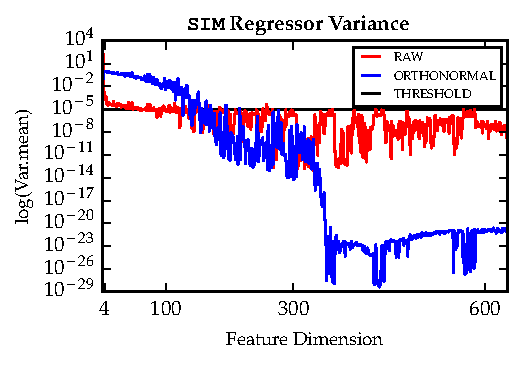
\includegraphics[scale=1]{Figures/SimDimensionSelectionRegLPP.pdf}
    }
    \caption[French \code{SIM} Regressor Variances]{The average of 9 fMRI run semantic regressor variances. There are 3 non-embedding regressors, and 634 \code{SIM}-based regressors. \code{RAW} stands for regressor values directly after hemodynamic convolution, \code{ORTHONORMAL} stands for de-linearized regressors after Gram-Schmidt process. \code{THRESHOLD} for regressor selection is fixed at \(10^{-5}\). The \code{RAW} regressors' variance declines dramatically after first few \code{SIM} regressors (dim > 3), and stays relatively stable for later dimensions. This observed trend corresponds well to the eigenvalue evolution of \code{SIM} space (Figures \ref{fig:SimDimensionSeletionVarRatio} and \ref{fig:FreDecorVarRatio}). \code{ORTHONORMAL} regressors's variance declines more slowly, and has a noised plateau around dimension 100 -- 300. Later regressors suffer more significantly in variance (smaller than \(10^{-23}\), approaching the computation precision limit of Python \code{float}s) and retained almost no information for the second half PCs. The threshold is cut around the upper bound of the \code{ORTHONORMAL} variance plateau noise, so a continuous regressor set could be included in the final design matrix without surpassing the dimensionality limit (of 200 which is the dimensionality of the used DepGlove embedding).} 
    \label{fig:freSIMRegVar}
\end{figure}


\subsection{Choice of \(\alpha\) and Effective Feature Dimensionality}

For each of four semantic models, we generated design matrices for each fMRI session with 103 or 203 features (including 3 non semantic embedding features). 

Analysis in Section \ref{appsubsec:alphadim} suggests that our research space for \(\alpha\) and feature-dimension parameters are complete: the distribution of voxel-configurations are bounded by our search space (see Figure \ref{fig:MIX_HeatmapAlphaDimS1R0} for the \code{MIX} distribution of subject 1 for an example, session-wise distribution plotting for all models are available online [TODO, add url]). 

Section \ref{appsubsec:alphadim} also illustrates the interaction between \(\alpha\) values and voxel regression performances, it confirms that a uniform \(\alpha\) setting penalizes certain cognitive models thus creating an important bias for model selection (see Section \ref{sec:ridgemethod}), supporting our choice of voxel-wise \(\alpha\) configuration.

\begin{figure}
\centering
        \makebox[.5\linewidth]{
            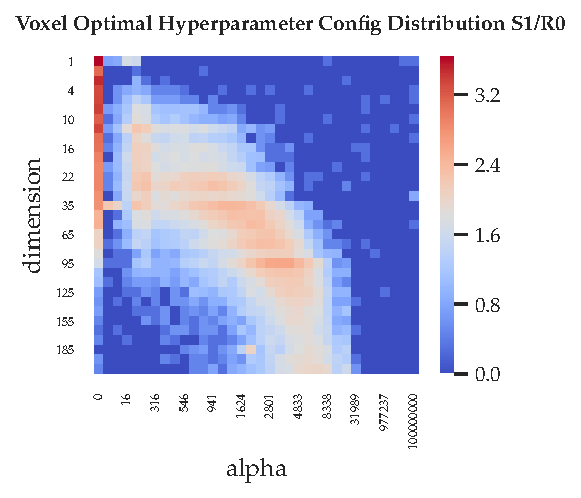
\includegraphics[scale=.8]{Figures/MIX_HeatmapAlphaDimS1R0.pdf}
            }
            \caption[Subject Best Hyper-parameter Configuration Voxel-Count Heat-map]{After averaging \code{MIX} best \code{r2}s across 9 runs of one same subject, best hyper-parameter configuration appears to be regularly distributed in the search space. A large proportion of voxels are best modeled with no Ridge regularization (especially for voxels using <4 features). Voxel-models requiring for higher-dimensional features are associated with larger \(\alpha\) values. A diagonal trend is found bounding  \(\alpha\). \(\alpha > 10^{4.5} (31989)\) rarely achieves best predictive performances, suggesting that the \(\alpha\) search space is complete for the subject.} 
            \label{fig:MIX_HeatmapAlphaDimS1R0}
\end{figure}

\section{Cognitive Analysis of fMRI Encoding}

For convenience, the voxel-model predictive performance is considered as voxel activations in response to different feature sets. 

\subsection{Non Semantic-Embedding Models}

%Contrast Map
\begin{figure}
    \centering
    \makebox[\linewidth]{
    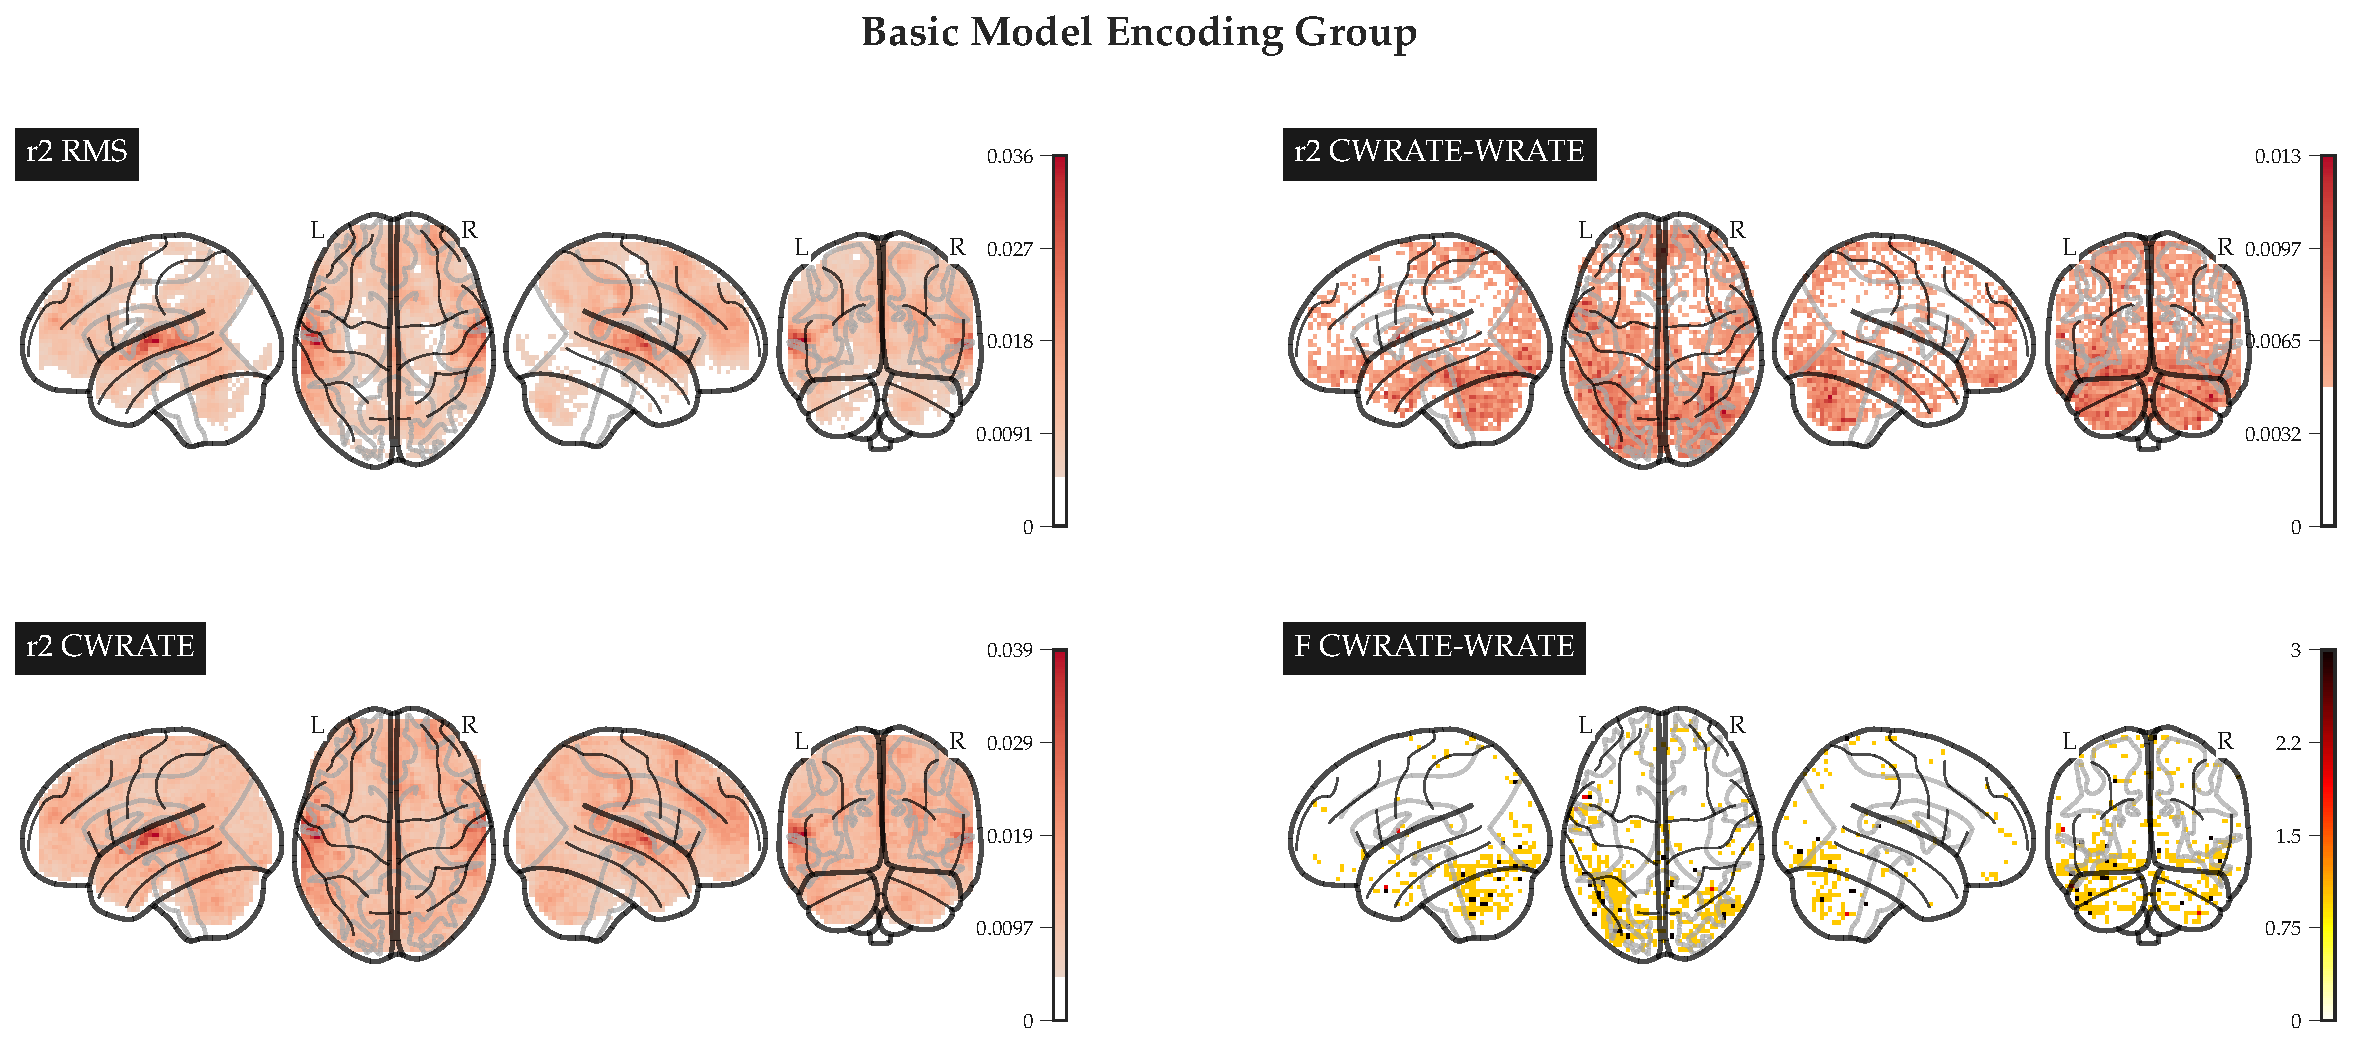
\includegraphics[width=.8\paperwidth]{Figures/BASE_ContrastMapG.pdf}
    }
    \caption[Encoding with \code{BASE} Features, Group]{\textbf{Left panels} are plots of voxel-wise \code{r2} scores for three \emph{classes} of non semantic-embedding regressors. With \code{RMS}, \code{WRATE} and \code{CWRATE}, consistent model performances are found for bilateral primary auditive cortices, with a slight preference for left hemisphere (Table \ref{tab:rmsCluters}). \textbf{Right upper and mid panels} are \code{r2} difference maps between two regressor classes. \code{WRATE} does not improve any voxel performance, and \code{CWRATE} improvements are mainly located in bilateral TP, MTG, ITG, frontopolar PFC and cerebellum near Fusiform cortex (Table \ref{tab:cwrateImprovementClusters}). \textbf{Right lower panel} is the F-test contrasting \code{RMS+WRATE+CWRATE} and \code{RMS+WRATE}. 3 levels of significance \code{1, 2, 3} are shown on the whole-brain map, corresponding respectively to p-values of uncorrected 0.05, 0.001 and voxel-wise corrected 0.05. The locations of the significant voxels are reported in Table \ref{tab:Ftest}.} 
    \label{fig:BASE_ContrastMapG}
\end{figure}

%r2 histogram
\begin{figure}
    \centering
    \makebox[\linewidth]{
    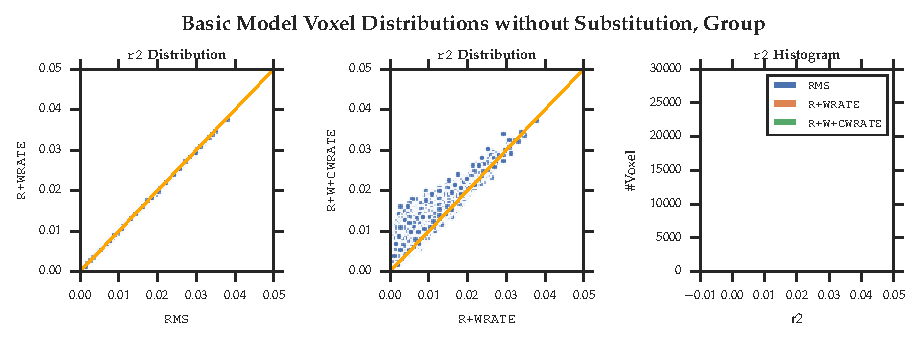
\includegraphics[width=\textwidth]{Figures/BASE_r2_Distribution.pdf}
    }
    \caption[Histogram of \code{r2} with \code{BASE} Features]{The voxel scores are averaged over all cross-validations of all subjects. \textbf{Left panel} shows that the addition of \code{WRATE} does not improve any voxel's model performance. \textbf{Mid panel} suggests that \code{CWRATE} slightly overfits a small portion of voxels, the improvement for most voxels are minute. \textbf{Right panel}: However for originally randomly-modeled voxels (x-axis from 0--0.01), \code{CWRATE} does bring significant improvements. The effect of model substitution is not pronounced in group average. However, subject-wise results are significantly higher (up to 0.2) and the score variability and overfitting are more remarkable.} 
    \label{fig:histo_base_best_nonsub_G}
\end{figure}

%clusters
% \begin{figure}
%     \centering
%     \makebox[\linewidth]{
%     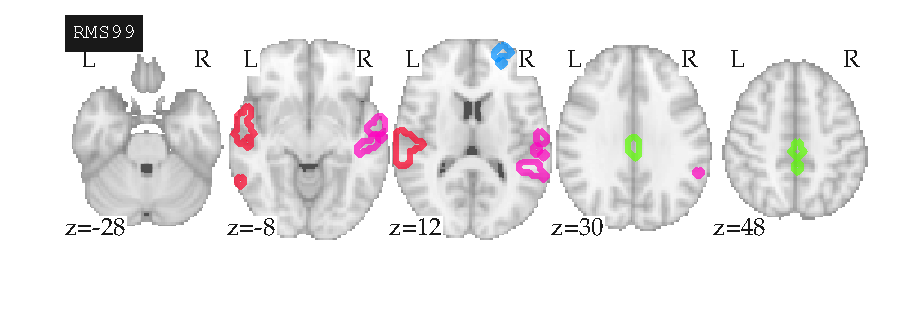
\includegraphics[width=.5\paperwidth]{Figures/RMS99_ClusterG.pdf}
%     }
%     \caption[\code{RMS} Top 1\% Voxel Clusters, Group]{[TODO remove?] With \code{RMS}, the best 1\% modeled voxels (with \code{r2}>0.0240) form 4 clusters containing more than 47 voxels. The two most large clusters are located in bilateral primary auditory cortices (BA41), a slight left-hemisphere preference is found (Left best \code{r2} 0.0362, cluster size 410 voxels, versus right best \code{r2} 0.0328 cluster size 337). Other two smaller clusters are located in right mid cingulum and right mid frontal cortex. The four-cluster structure is stable across \code{RMS}, \code{WRATE}, \code{CWRATE} and \code{SIM} \emph{feature classes}.} 
%     \label{fig:RMS99_ClusterG}
% \end{figure}

\begin{table}
    \small
    \centering
    \begin{ThreePartTable}
    \begin{tabularx}{\textwidth}{p{1.8cm}p{.5cm}p{1.4cm}p{1cm} *{6}{r}}
    \mc{6}{l}{\tabhead{\code{RMS/CWRATE/SIM/ASN} Best Modeled Voxel Clusters}} \\
    \toprule
    \tabhead{Position} & \tabhead{BA} & \tabhead{Functional Label} & \tabhead{Feature Class} & \tabhead{x} & \tabhead{y} & \tabhead{z} & \tabhead{\#Voxel} & \code{r2} \tabhead{Peak} & \code{r2} \tabhead{Min} \\
    \toprule
    \mc{3}{l}{\tabhead{Top .1\%}} \\
    \midrule
    \mr[t]{3}{=}{Temporal Sup L} & \mr[t]{3}{=}{41} & \mr[t]{3}{=}{Prim Auditory} &  \code{RMS} &  -59 & -13 & 6 &  56 & .0362 &  .0240 \\ 
    & & & \code{CWRATE} & -61 & -12 & 4 & 61 &.0387 &  .0259\\
    & & & \code{SIM} & -60 & -13 & 6 & 53 & .0412 &  .0291 \\
    & & & \code{SIG} & -61 & -11 & 4 & 87 & .0430 & .0301\\
    & & & \code{ASN} & -60 & -13 & 6 & 53 & .0388 &  .0293 \\
    \midrule
    \midrule
    \mc{7}{l}{\tabhead{Top 1\%}}   \\
    \midrule
    \mr[t]{3}{=}{Temporal Sup L} & \mr[t]{3}{=}{41} & \mr[t]{3}{=}{Prim Auditory} & \code{RMS} & -60 & -12 & 4 & 410 & .0362 &  .0150 \\
    & & & \code{CWRATE} & -60 & -11 & 4 & 417 &.0387 &  .0178\\
    & & & \code{SIM} & -60 & -11 & 3 & 522 &.0413 &  .0214\\
    & & & \code{SIG} & -61 & -17 & 4 & 527 &.0430 &  .0301\\
    & & & \code{ASN} & -60 & -19 & 4 & 515 &.0388 &  .0218\\
    \midrule
    \mr[t]{3}{=}{Cingulum Mid R} & \mr[t]{3}{=}{23} & \mr[t]{3}{=}{-} & \code{RMS} & 0 & -24 & 29 & 69& .0189 & .0150\\
    & & & \code{CWRATE}&  1 &  -23 & 29 & 55 &.0202 &  .2587\\
    & & & \code{SIM}& 2 & -24 & 44 & \textbf{37}\tnote{1} & .0243 &  .0214 \\
    & & & \code{SIG} & 2 & -25 & 45 & 55 &.0250 &  .0301\\
    & & & \code{ASN} & -\tnote{2} \\

\midrule
    \mr[t]{3}{=}{Frontal Mid R} & \mr[t]{3}{=}{10} & \mr[t]{3}{=}{-} & \code{RMS} &  29 & 56 & 20 & 103 & .0180 &  .0150\\
    & & & \code{CWRATE} & 28 &  60 & 19 & 55 &.0221 &  .0178\\
    & & & \code{SIM} & 29 & 59 & 19 & 92 &.0256 &  .0214\\
    & & & \code{SIG} & 26 & 57 & 20 & 86 &.0252 &  .0301\\
    & & & \code{ASN} & 30 & 59 & 19 & 74 &.0259 &  .0218\\

\midrule
    \mr[t]{3}{=}{Temporal Sup R} & \mr[t]{3}{=}{41} & \mr[t]{3}{=}{Prim Auditory} & \code{RMS} & 61 & -13 & 2 & 337 & .0328 &  .0150\\
    & & & \code{CWRATE} &  62 & -11 & 3  & 198 &.0342 &  .0178\\
    & & & \code{SIM} & 62 & -9 & 1 & 264 &.0366 &  .0214\\
    & & & \code{SIG} & 61 & -11 & 3 & 262 &.0402 &  .0301\\
    & & & \code{ASN} & 62 & -13 & 3 & 266 &.0370 &  .0218\\


\bottomrule
    \end{tabularx}
    \begin{tablenotes}
    \footnotesize
    \item Coordinates are reported in Montreal Neurological Institute (MNI) standardized spaces.
    \item[1] Cluster size smaller than 47 voxels, 1500 \(\text{mm}^3\).
    \item[2] Cluster not found. 
\end{tablenotes}  
\end{ThreePartTable}
\caption[\code{RMS/CWRATE/SIM/SIG/ASN} Best Modeled Voxel Clusters]{Across four regressor classes, the best models voxels are consistently found in four cortical areas: bilateral pSTG (BA41, primary auditory), right mid cingulate cortex (MCC) and right aPFC (BA10). The most severe voxel score selection leads to left primary cortex (BA41) activation. With the addition of semantic features including \code{CWRATE}, \code{SIM} and \code{ASN}, left pSTG cluster grows while right MCC shrinks. \code{CWRATE} penalizes voxels in right BA10 and BA41, while semantic regressors re-improves the scores. With \code{ASN}, a significant left pSTG cluster centroid posterior shift is observed. No other contrasting differences are found for \code{SIM} and \code{ASN}.\label{tab:rmsCluters}}
% The shrinkage of Mid Cingulum's proportion in top 1\% voxel models might imply that it has a limited participating in \similarity processing.
\end{table}
\begin{table}
    \small
    \centering
    \begin{ThreePartTable}
    \begin{tabularx}{\textwidth}{l l p{1.5cm} *{3}{r} *{2}{P{1.2cm}}P{1.4cm}}
    \mc{6}{l}{\tabhead{\code{CWRATE} Best Improved Voxel Clusters}} \\
    \toprule
    \tabhead{Position} & \tabhead{BA} & \tabhead{Functional Label} & \tabhead{x} & \tabhead{y} & \tabhead{z} & \tabhead{\# Voxel} & \(\Delta\)\code{r2} \tabhead{Peak} & \(-\log_{10}\)\tabhead{ p-value} \\
    \toprule
    \mc{7}{l}{\tabhead{Top 2\%}}  &  >.0067 & >3.66   \\
    \midrule
    Temporal Pole Mid L & 38 & - & -53 & 11 & -33 & 22 & .0118 & 4.18 \\
Temporal Inf L & 37 & Fusiform & -47 & -43 & -24 & 90 & .0114 &  4.18\\
Rectus L & 11 & - & -5 & 46 & -26 & 16 & .0110 & 4.00 \\
Cerebelum Crus2 R & 37 & Fusiform & 45 & -69 & -38 & 89 & .0130 & 4.35\\
\bottomrule
    \end{tabularx}
    % \begin{tablenotes}
    % \footnotesize
    % \item[1] A cosine distance near 0 indicates a greater similarity.
% \end{tablenotes}  
\end{ThreePartTable}
\caption[\code{CWRATE} Voxel Improvement Clusters]{The most severe voxel score selection of \code{RMS} leads to left primary cortex (BA41) activation. Also well modeled voxels are distributed in more extensive areas of bilateral BA41 and right BA23 and BA10. With the addition of \code{CWRATE} features, voxel performances are systematically improved. With \code{CWRATE}, no other clusters appear in the thresholded voxel set. Left BA41 has a higher concentration of best modeled voxels, while right BA41 and right mid cingulum degrade in voxel score ranking. Right BA10 also improves in ranking. \label{tab:cwrateImprovementClusters}}
\end{table}

Figure \ref{fig:BASE_ContrastMapG} illustrates the group-wise results for non-semantic-embedding feature classes. Subject-wise results are available online\footnote{\url{http://bit.ly/micipsa_base_wholebrain}}. Additionally, Figure \ref{fig:histo_base_best_nonsub_G} shows the exact impact on addition of \code{WRATE} and \code{CWRATE} \emph{feature groups} to the design matrix, without substituting worse nesting-model results with better nested-model results. Subject-wise results are available online\footnote{\url{http://bit.ly/micipsa_regression_histogram}}, the overfitting with feature additions are more pronounced.

\code{RMS} preferentially models primary auditory cortical activities in Broadmann Area (BA) 41, together with other two clusters located in right mid cingulum and right middle frontal cortex (Table \ref{tab:rmsCluters}). The addition of \code{WRATE} does not bring any impact (Figure \ref{fig:histo_base_best_nonsub_G} left panel), possibly due to the high co-linearity with \code{RMS} by definition, thus the orthonormalized feature contains only uninformative noises despite a relatively important variance (0.96 after orthonormalization, \code{CWRATE} has only 0.10 for reference). With \code{CWRATE}, an extensive range of voxels distributed in the whole brain received better performance (Figure \ref{fig:histo_base_best_nonsub_G} middle panel). 

A left-hemisphere preference for textual listening comprehension is suggested: left primary auditory cortex (BA41) is better modeled than in right hemisphere with \code{RMS} and \code{CWRATE}. On adding \code{CWRATE}, the imbalance between left and right BA41 is enlarged. Table \ref{tab:cwrateImprovementClusters} reports 4 clusters containing more than 16 voxels that are improved (W=136, \(\Delta\)\code{r2}>0.0067, p-value<\(10^{-3.66}\) uncorrected) in left BA37 (MTP), bilateral BA37 (Fusiform Gyrus) and left Rectus. The Wald F-test on \code{CWRATE} contrast reports isolated voxels surviving voxel-wise multi-comparison significance test (Table \ref{tab:Ftest}, p-value<0.05 voxel-wise multi-comparison corrected). The voxels are mainly located in bilateral BA37, left BA18, 19. 


\subsection{\emph{Similarity} Nested Model}

\begin{figure}
    \centering
    \makebox[\linewidth]{
    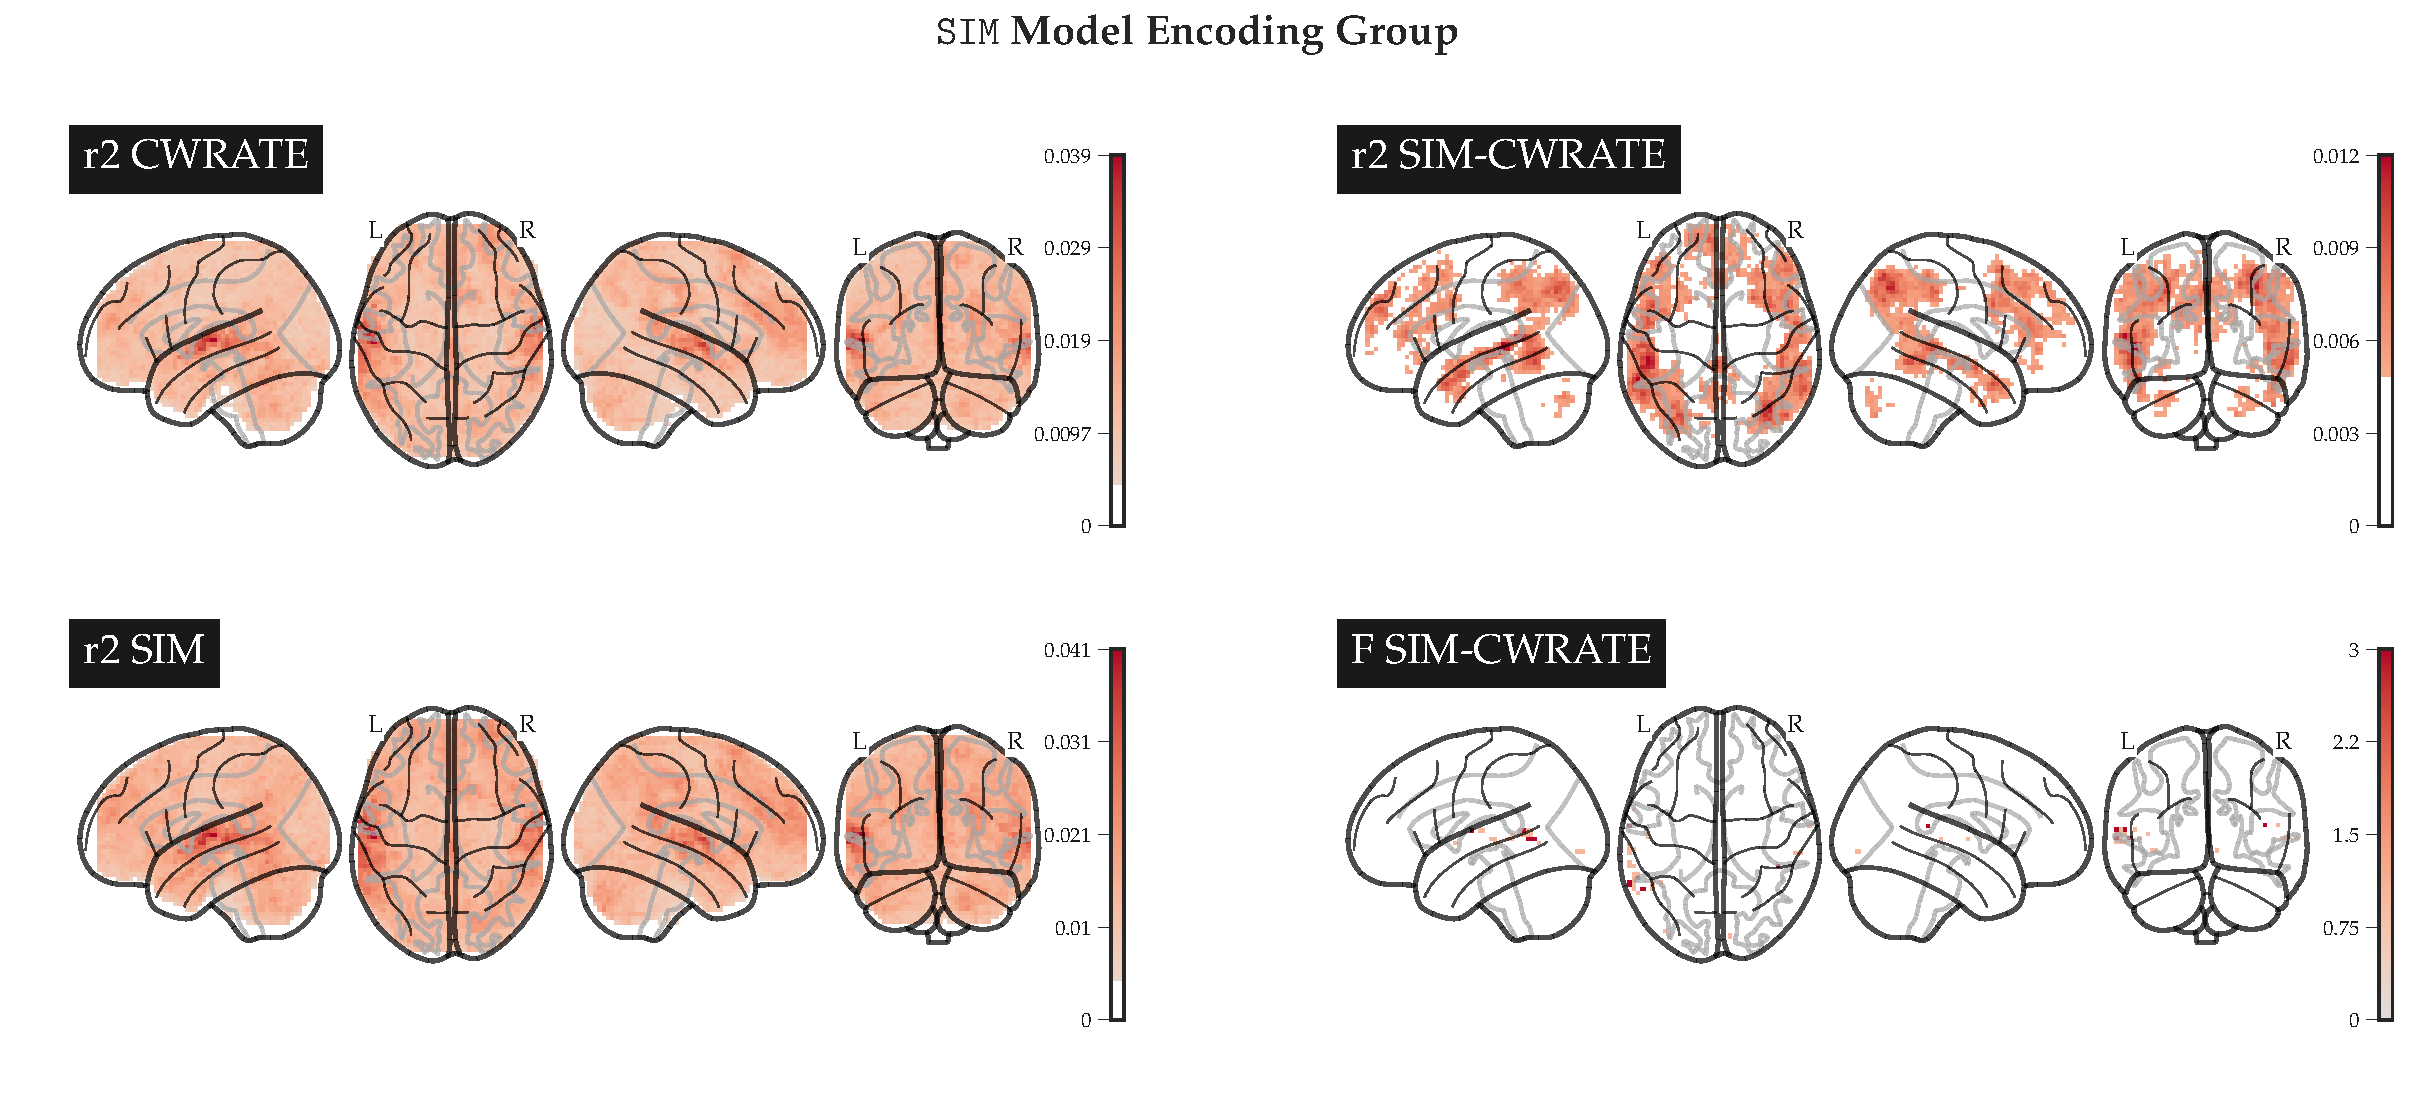
\includegraphics[width=.8\paperwidth]{Figures/SIM_ContrastMapG.pdf}
    }
    \caption[Encoding with \code{SIM} Features, Group]{\textbf{Left panels}: The global activation pattern is unchanged with the feature addition. Best modeled zones are bilateral primary auditory cortices. \textbf{Right upper panel}  shows that \code{SIM} better models bilateral MTG, sup Parietal, Angular Gyrus (part of Wernicke's area), supramarginal gyrus and prefrontal areas (Table \ref{tab:simImprovementClusters}). F-test in \textbf{right lower panel} reports significant voxels in left pMTG BA21, 39, right pSTG BA22 and left Heschl BA4 (Table \ref{tab:Ftest}). Subject-wise results are available online at \url{http://bit.ly/micipsa_sim_wholebrain}.} 
    \label{fig:SIM_ContrastMapG}
\end{figure}

\begin{figure}
    \centering
    \makebox[\linewidth]{
    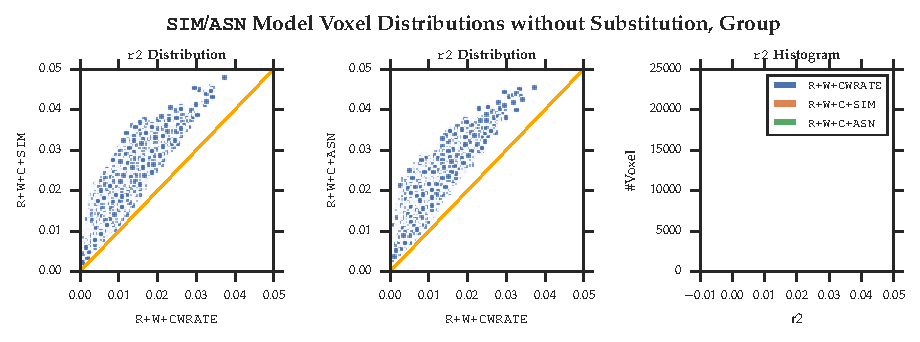
\includegraphics[width=.8\paperwidth]{Figures/SIM_ASN_Distribution.pdf}
    }
    \caption[Histogram of \code{r2} with \code{SIM/ASN} Features]{The group average of semantic embedding models make both important contributions for voxel-modeling (\textbf{left} and \textbf{mid} panels). \textbf{Right} panel shows that \code{ASN} model scores are distributed around a higher average (0.014) than \code{SIM} (0.01). Subject-wise results are available online at \url{http://bit.ly/micipsa_regression_histogram}.} 
    \label{fig:SIM_ASN_Distribution}
\end{figure}

\begin{table}
    \small
    \centering
    \begin{ThreePartTable}
    \begin{tabularx}{\textwidth}{l l p{1.5cm} *{3}{r} *{2}{P{1.2cm}}P{1.4cm}}
    \mc{6}{l}{\tabhead{\code{SIM} Best Improved Voxel Clusters}} \\
    \toprule
    \tabhead{Position} & \tabhead{BA} & \tabhead{Functional Label} & \tabhead{x} & \tabhead{y} & \tabhead{z} & \tabhead{\# Voxel} & \(\Delta\)\code{r2} \tabhead{Peak} & \(-\log_{10}\)\tabhead{ p-value} \\
    \toprule
    \mc{7}{l}{\tabhead{Top .5\%}}  &  >.0079 & >4.35   \\
    \midrule
    Temporal Mid L & 21 & - & -51 & -34 & 1 & 86 & .0119 &4.35\\
Parietal Sup L & 7 & - & -27 & -72 & 44 & 17 & .0099 &4.35\\
Angular R & 39 & - & 35 & -65 & 44 & 49 & .0114 &4.35\\
Temporal Mid R & 21 & - & 57 & -36 & -0 & 17 & .0098 &4.35\\
\bottomrule
    \end{tabularx}
    % \begin{tablenotes}
    % \footnotesize
    % \item[1] A cosine distance near 0 indicates a greater similarity.
% \end{tablenotes}  
\end{ThreePartTable}
\caption[\code{SIM} Voxel Improvement Clusters]{We thresholded Wilcoxon signed-rank test's significance at \(10^{-4.35}\) as a clean cut is found in p-value histogram, which leads to a selection of top .5\% important voxel-model improvements. The largest and most improved voxel-cluster is found in left BA21, then in right angular gyrus which is part of Wernicke's area. A more lateral and smaller-cluster improvement is found in right MTG. \label{tab:simImprovementClusters}}
\end{table}

%(language, V. S. Ramachandran, and Edward Hubbard published a paper in 2003 metaphors for angular 

We added with upon non semantic-embedding models \code{SIM} freatures to construct \similarity semantic models. While the whole-brain activation pattern stays globally unchanged (Figure \ref{fig:SIM_ContrastMapG} for group-wise average), in \code{SIM} voxel-models, left primary cortex are better ranked than in \code{BASE} model, while right mid cingulum models degrade (Table \ref{tab:rmsCluters}). \code{SIM} enlarges the performance superiority of left STG over right STG, indicating a left preference for textual semantic \similarity processing. The shrinkage of Mid Cingulum's proportion in top 1\% voxel models might imply that it has a limited participating in \similarity processing. The \code{r2} distribution analysis (Figure \ref{fig:SIM_ASN_Distribution} left) shows that in group-average \code{SIM} is informative for most of the voxel-models and none of voxels is overfitted by this addition. Table \ref{tab:simImprovementClusters} reports the most improved voxel clusters by \code{SIM} to be located in bilateral MTG, left Sup Parietal and right Angular Cortex (W=210, \(\Delta\)\code{r2}>0.0079, p<\(10^{-4.35}\) uncorrected). Left MTG improvements are more extensive and more important than right MTG. F-test results shows that \code{SIM} significantly improves isolated voxels (Table \ref{tab:Ftest}, p<0.05 voxel-wise multi-comparison corrected) in left pMTG BA21, 39, right pSTG BA22.

\subsubsection{\emph{Similarity} Nested Model with \code{SIG}}

\code{SIG} contrasts with \code{CWRATE} class models gave similar contrast maps as \code{SIM}: bilateral IFGtri, MTG and ITG, SPG and AG are found. With \code{SIG} the left ITGtri and left ITG improvements are more drastic. A more detailed presentation of \code{SIG} results is available in Section \ref{subsec:sig}.

\subsection{\emph{Association} Nested Model}

\begin{figure}
    \centering
    \makebox[\linewidth]{
    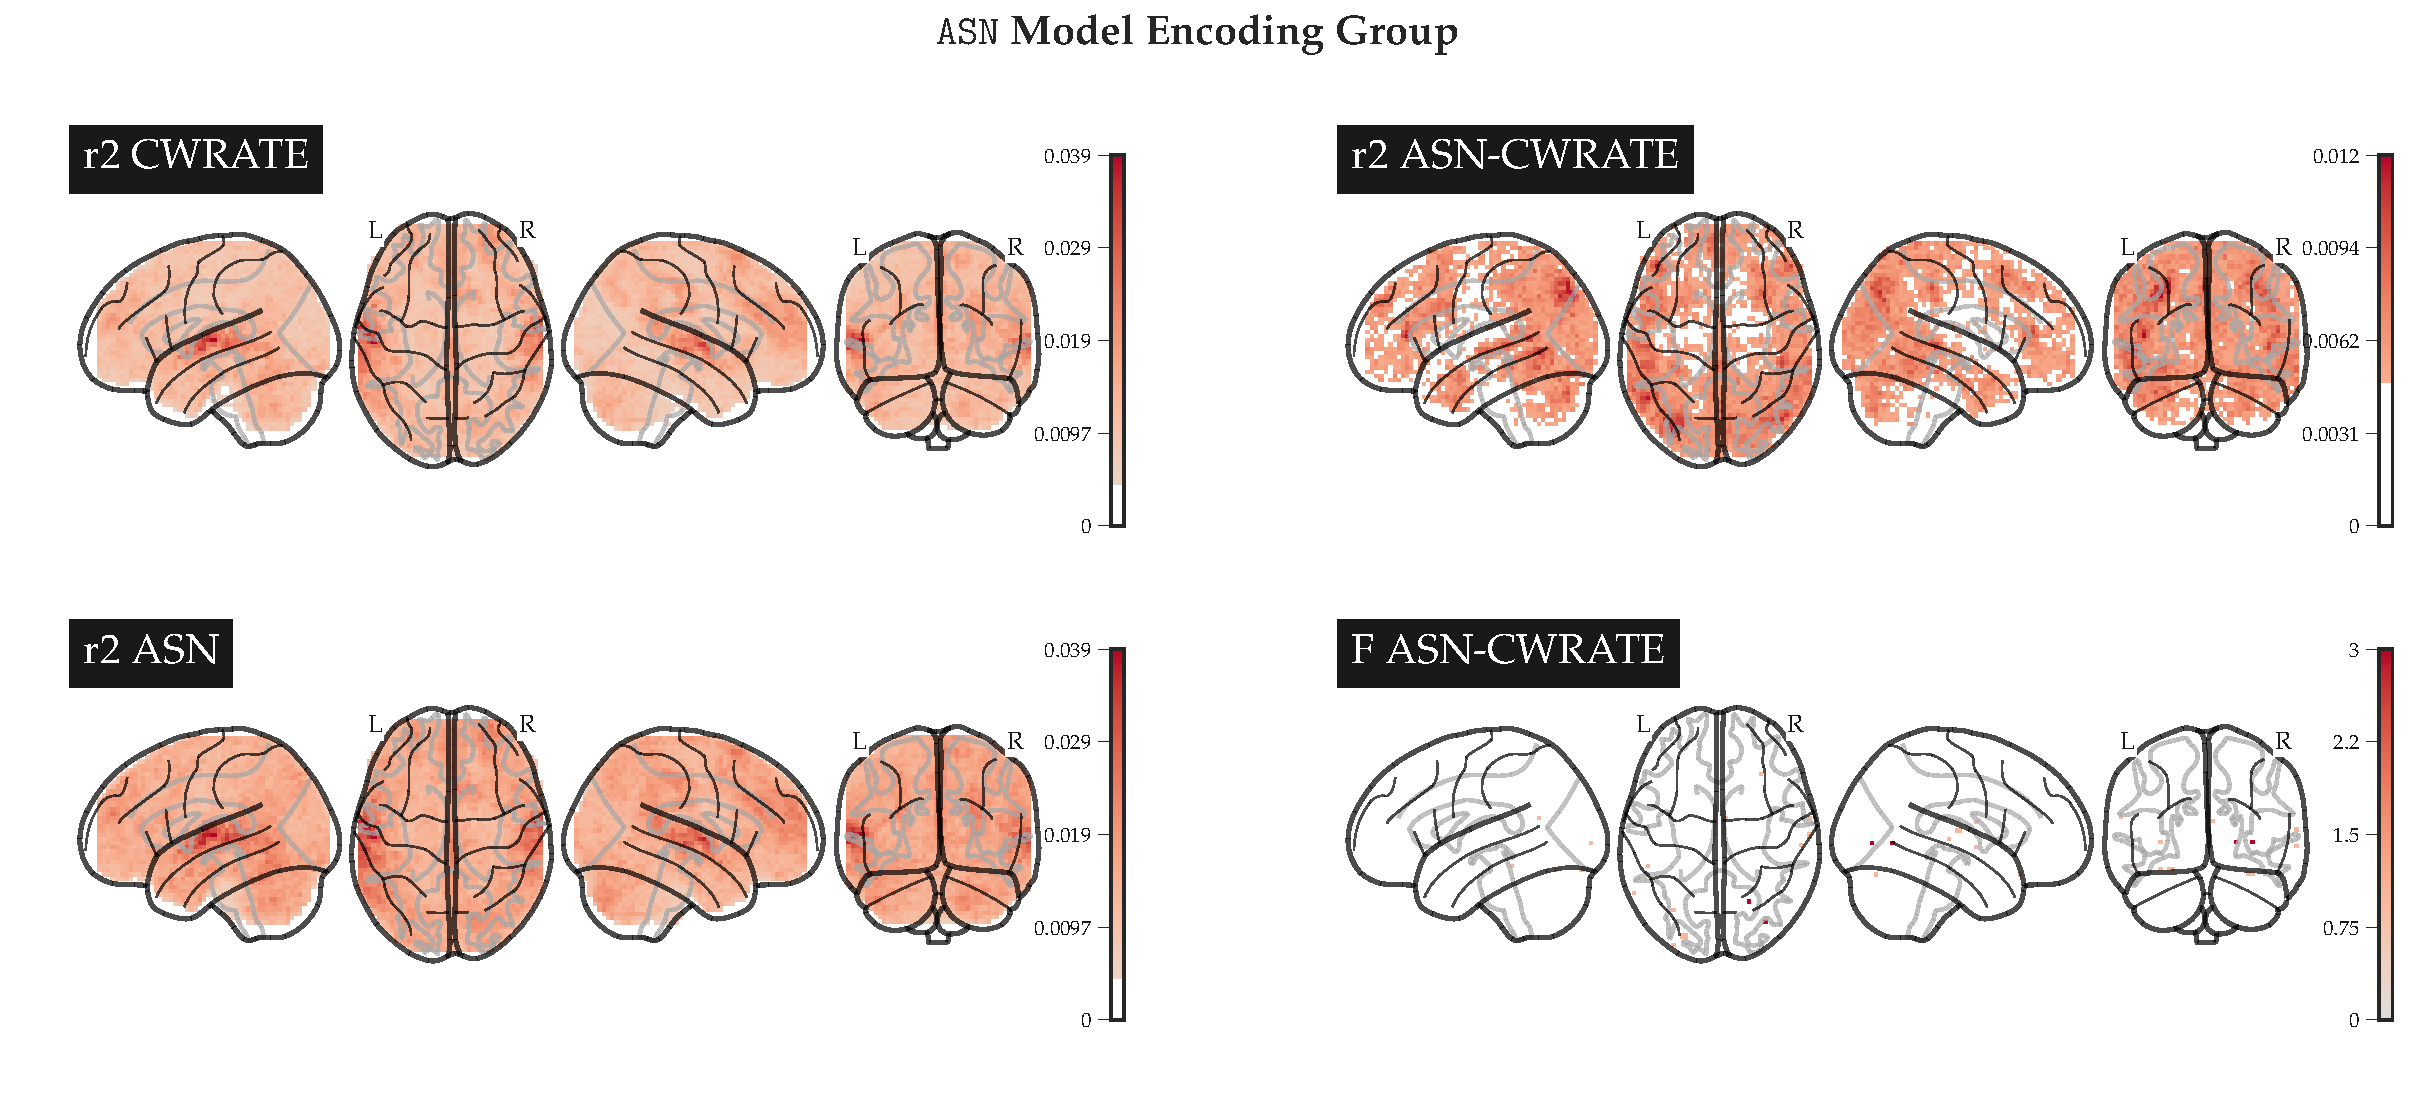
\includegraphics[width=.8\paperwidth]{Figures/ASN_ContrastMapG.pdf}
    }
    \caption[Encoding with \code{ASN} Features, Group]{\textbf{Left panels}: Consistent with former results, the addition of \code{ASN} on \code{BASE} regressors does not change the bilateral primary auditive cortices' dominance. Improvements of voxel-models are distributed in an extensive part of all lobes (\textbf{right upper panel}). The most improved voxels are located in bilateral MTG, IFGtri, mid occipital cortex, angular gyrus, sup/mid frontal cortex, mid cingulum  (Table \ref{tab:asnImprovementClusters}). F-test in \textbf{right lower panel} reports significant voxels in right lingual BA19 and mid occipital area BA18 (Table \ref{tab:Ftest}). Subject-wise results are available online at \url{http://bit.ly/micipsa_asn_wholebrain}.} 
    \label{fig:ASN_ContrastMapG}
\end{figure}


On addding \code{ASN} features on \code{BASE} features, the bilateral auditive cortices dominance is consistently kept (Figure \ref{fig:SIM_ContrastMapG} for group-wise average). The contribution brought by \code{ASN} on top 4 voxel-clusters initially found by \code{RMS} model is similar to \code{SIM} (Table \ref{tab:rmsCluters}): improvement in bilateral Prim Auditory with a slight left preference, shrinkage of right MCingulum and slight improvement of frontopolar PFC. These clusters therefore do not show an observable preference for \code{SIM} and \code{ASN}.

\code{ASN} brings voxel-model performance boost in an extensive cortical regions. The Wilcoxon test shows near-significant performance improvements (W=190, \(\Delta\)\code{r2}>0.0065, p-value<\(10^{-4.18}\) uncorrected) in left BA39 (visual), right angular gyrus (associated with aphasia), right BA21 MTG, left BA37 fusiform gyrus (Table \ref{tab:asnImprovementClusters}). F-test results shows that \code{ASN} significantly improves isolated voxels (Table \ref{tab:Ftest}, p-value<0.05 voxel-wise multi-comparison corrected) in right lingual gyrus BA19 and BA18 (visual association).
 % right BA21 MTG [Senkowski, D., Schneider, T. R., Foxe, J. J., and Engel, A. K. (2008)., multisensory capabilities] Fusiform [within category Trafton, A. "How does our brain know what is a face and what’s not?" MIT News]
\subsection{\emph{Similarity}/\emph{Association} Contrast}

\subsubsection{With \code{SIM}}

\begin{figure}
    \centering
    \makebox[\linewidth]{
    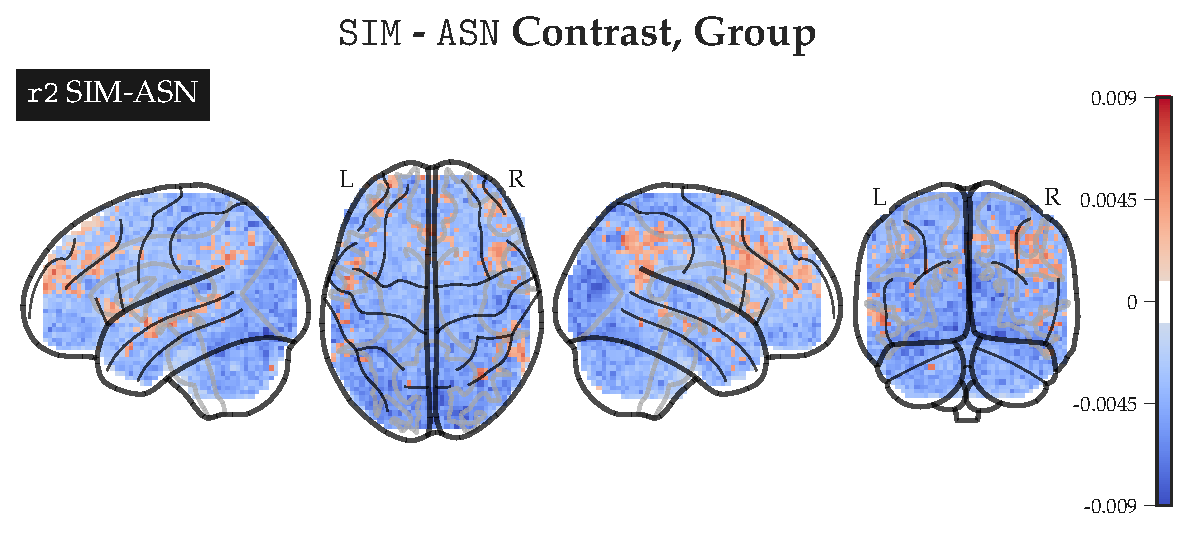
\includegraphics[width=.4\paperwidth]{Figures/EMB_SIM_ASN_r2_ContrastMapG.pdf}
    }
    \caption[\code{SIM}-\code{ASN} Contrast, Group]{The differences of best voxel-model \code{r2}s are plotted. \code{SIM} preference is found in left BA10 Superior PFC, left anterior cingular cortex, left STS, left medial PFC, right IPL, right STG, MTG (Table \ref{tab:simasnContrastClusters_sim}). \code{ASN} preferences are found in bilateral BA18, right BA20, left BA7, 19, 37 (visual association, primary visual, parahippocampal). Subject-wise results are available online at \url{http://bit.ly/micipsa_sim_asn_contrast}} 
    \label{fig:EMB_SIM_ASN_ContrastMapG}
\end{figure}

\begin{table}
    \small
    \centering
    \begin{ThreePartTable}
    \begin{tabularx}{\textwidth}{l l p{1.4cm} *{3}{r} *{2}{P{.8cm}} P{1.3cm} P{.5cm}}
    \mc{6}{l}{\tabhead{\code{SIM-ASN} Voxel Contrast, Preference for \code{SIM}}} \\
    \toprule
    \tabhead{Position} & \tabhead{BA} & \tabhead{Functional Label} & \tabhead{x} & \tabhead{y} & \tabhead{z} & \tabhead{\# Voxel} & \(\Delta\)\code{r2} \tabhead{Peak} & \(-\log_{10}\)\tabhead{ p-value} & \tabhead{Cluster ID} \\
    \toprule

    Frontal Sup L  &  10  &  -  &  -27  &  59  &  25  &  4  &   .0073  &  6.75  &  1 \\
    Cingulum Ant L  &  32  &  -  &  -8  &  34  &  25  &  5  &   .0069  &  6.15  &  2 \\
    \midrule
    Temporal Sup L  &  22  &  -  &  -55  &  -1  &  -7  &  3  &   .0062  &  5.35  &  3 \\
    Frontal Mid L  &  10  &  -  &  -36  &  49  &  15  &  4  &   .0061  &  5.29  &  4 \\
    Cingulum Ant L  &  32  &  -  &  -2  &  30  &  31  &  2   &   .0061  &  5.24  &  5 \\
    Parietal Inf R  &  40  &  -  &  46  &  -49  &  44  &  10  &   .0059  &  5.09  &  6 \\
    Angular R  &  39  &  -  &  33  &  -64  &  47  &  2   &   .0057  &  4.75  &  7 \\
    Precentral R  &  8  &  -  &  39  &  8  &  47  &  2   &   .0057  &  4.73  &  8 \\
    Caudate R  &  48  &  Caudate  &  17  &  21  &  3  &  2   &   .0052  &  4.20  &  9 \\
    Frontal Sup R  &  10  &  -  &  27  &  65  &  9  &  2   &   .0051  &  4.09  &  10 \\
    Temporal Sup R  &  39  &  -  &  65  &  -55  &  22  &  4  &   .0050   &  4.05  &  11 \\
    Frontal Mid L  &  10  &  -  &  -27  &  40  &  31  &  2   &   .0047  &  3.68  &  12 \\
    Temporal Mid R  &  22  &  -  &  49  &  -23  &  -7  &  2   &   .0046   &  3.66  &  13 \\
    Parietal Inf R  &  40  &  -  &  52  &  -42  &  53  &  4  &   .0045   &  3.55  &  14 \\
    Frontal Sup R  &  9  &  -  &  14  &  43  &  41  &  2   &   .0045   &  3.52  &  15 \\
    Angular R  &  39  &  -  &  39  &  -55  &  28  &  3   &   .0044   &  3.45   &  16 \\
    Temporal Mid L  &  38  &  -  &  -49  &  8  &  -26  &  2   &   .0043  &  3.26   &  17 \\
    Angular R  &  39  &  -  &  33  &  -68  &  50  &  2   &   .0042   &  3.22  &  18 \\
    SupraMarginal R  &  39  &  -  &  62  &  -49  &  28  &  2   &   .0042   &  3.20  &  19 \\
\bottomrule
    \end{tabularx}
    \begin{tablenotes}
    \footnotesize
    \item[] Voxel-wise Bonferroni corrected p=0.05 corresponds to uncorrected \(-\log_{10}\) p=6.04.
\end{tablenotes}  
\end{ThreePartTable}
\caption[\code{SIM-ASN} Voxel Contrast, \code{SIM}, Group]{The \code{SIM}-\code{ASN} contrast is computed by subtracting group-average voxel-wise \code{r2}. The significance is reported by two-tailed Wilcoxon signed-rank test before multi-comparison correction. The cluster is reported only if the average \code{r2} of \code{SIM} is higher than \code{ASN}. No cluster-size limit was applied when computing connected clusters. Significant small clusters are found in left superior frontal cortex and anterior cingulate cortex. Additional near-significant clusters are located in left superior temporal gyrus. No ventroanteriotemporal cluster is found for \code{SIM}. \label{tab:simasnContrastClusters_sim}}
\end{table}

\begin{table}
    \small
    \centering
    \begin{ThreePartTable}
    \begin{tabularx}{\textwidth}{l l p{1.5cm} *{3}{r} *{2}{P{.8cm}} P{1.3cm} P{.5cm}}

    \mc{6}{l}{\tabhead{\code{SIM-ASN} Voxel Contrast, Preference for \code{ASN}}} \\
    \toprule
    \tabhead{Position} & \tabhead{BA} & \tabhead{Functional Label} & \tabhead{x} & \tabhead{y} & \tabhead{z} & \tabhead{\# Voxel} & \(\Delta\)\code{r2} \tabhead{Peak} & \(-\log_{10}\)\tabhead{ p-value} & \tabhead{Cluster ID} \\
    \toprule
Cuneus R & 18 & VisualAssoc & 5 & -77 & 22 & 3 & .0083 & 9.99 & 1 \\
Cuneus L & 18 & VisualAssoc & 2 & -87 & 25 &  &  .0083 & 8.27 & 1a\tnote{*} \\
Calcarine L & 18 & VisualAssoc & 2 & -83 & 15 &  &  .0070 & 6.30 & 1b \\
Temporal Inf R & 20 & - & 46 & -17 & -26 & 2 &  .0090 & 9.21 & 2 \\
Cerebellum 6 L & 18 & VisualAssoc & -8 & -80 & -13 & 4 &  .0087 & 8.78 & 3 \\
Parietal Sup L & 7 & - & -27 & -71 & 56 & 2 &  .0086 & 8.70 & 4 \\
Occipital Mid R & 18 & VisualAssoc & 36 & -80 & 3 & 2 &  .0078 & 7.70  & 5 \\
Cerebellum 8 L & 37 & Fusiform & -21 & -55 & -45 & 3 &  .0078  & 7.67 & 6 \\
Occipital Mid L & 19 & - & -30 & -77 & 15 & 2 &  .0076 & 7.29  & 7 \\
Cerebellum Crus1 L & 18 & VisualAssoc & -2 & -80 & -16 & 2 &  .0075 & 7.16  & 8 \\
Fusiform R & 18 & VisualAssoc & 30 & -83 & -4 & 3 &  .0073  & 6.85  & 9 \\
Hippocampus R & 50 & Thalamus & 17 & -11 & -7 & 2 &  .0072 & 6.69 & 10 \\
Vermis 10 & 37 & Fusiform & -2 & -42 & -32 & 2 &  .0072 & 6.65 & 11 \\
Fusiform R & 19 & - & 33 & -71 & 3 & 2 &  .0072 & 6.64  & 12 \\
Fusiform L & 36 & Parahip & -33 & -26 & -19 & 2 &  .0071 & 6.45  & 13 \\
Thalamus L & 50 & Thalamus & -2 & -20 & 3 & 2 &  .0070  & 6.36 & 14 \\
Calcarine L & 18 & VisualAssoc & -27 & -64 & 6 & 3 &  .0069  & 6.24  & 15 \\
Calcarine R & 17 & PrimVisual & 17 & -83 & 6 & 2 &  .0069  & 6.22 & 16 \\
Calcarine R & 17 & PrimVisual & 11 & -80 & 9 & 2 &  .0069  & 6.20 & 17 \\
Cerebellum 6 R & 19 & - & 14 & -64 & -13 & 2 &  .0068 & 6.04  & 18 \\
\midrule
Occipital Mid R & 18 & VisualAssoc & 30 & -93 & 15 & 2 &  .0068 & 6.02  & 19 \\
Parietal Inf L & 40 & - & -30 & -39 & 37 & 2 &  .0068 & 6.01 & 20 \\
Calcarine R & 17 & PrimVisual & 5 & -64 & 15 & 2 &  .0067& 5.94  & 21 \\
Calcarine L & 17 & PrimVisual & 2 & -87 & 6 & 4 &  .0067 & 5.88 & 22 \\
Occipital Mid L & 19 & - & -39 & -74 & 6 & 2 &  .0066 & 5.79 & 23 \\
Calcarine R & 17 & PrimVisual & 11 & -68 & 15 & 2 &  .0066 & 5.79 & 24 \\
Cerebellum 8 R & 37 & Fusiform & 30 & -64 & -54 & 2 &  .0066 & 5.76 & 25 \\
Cerebellum 9 L & 37 & Fusiform & -11 & -42 & -32 & 2 &  .0066 & 5.75& 26 \\
Calcarine L & 17 & PrimVisual & -8 & -87 & 3 & 2 &  .0065 & 5.66 & 27 \\
Lingual L & 19 & - & -14 & -45 & -7 & 2 &  .0063 & 5.45 & 28 \\
Temporal Mid L & 20 & - & -39 & -4 & -26 & 2 &  .0060 & 5.21 & 29 \\
Calcarine L & 18 & VisualAssoc & -8 & -96 & -13 & 2 &  .0060 & 5.12 & 30 \\
\bottomrule
    \end{tabularx}
    \begin{tablenotes}
        \footnotesize
        \item[] Voxel-wise Bonferroni corrected p=0.05 corresponds to uncorrected \(-\log_{10}\) p=6.04.
        \item[*] Sub-peaks in one same cluster. 
    \end{tablenotes}  
\end{ThreePartTable}
\caption[\code{SIM-ASN} Voxel Contrast, \code{ASN}, Group]{The \code{SIM}-\code{ASN} contrast is computed by subtracting group-average voxel-wise \code{r2}. The significance is reported by two-tailed Wilcoxon signed-rank test before multi-comparison correction. The cluster is reported only if the average \code{r2} of \code{ASN} is higher than \code{SIM}. No cluster-size limit was applied when computing connected clusters. \code{ASN}'s model advantage over \code{SIM} is often found in bilateral visual association and primary visual areas. Clusters in ventroposterior aspects of temporal lobe is also found in right fusiform, parahippocamal gyri. \label{tab:simasnContrastClusters_asn}}
\end{table}




Section \ref{appsubsec:nonnestedcompres} suggests that first feature dimensions of \code{SIM} can be partially recovered by \code{ASN} model. Therefore, \code{ASN} might also be able to model voxels using less than 5 features from \code{SIM}, the result might thus lack low-level \code{SIM}/\code{ASN} contrast. As the first 4 dimensions of \code{SIM} encodes primarily POS information (Section \ref{appsubsec:projectorvisu}), we performed ad-hoc regressions on \code{SIM} space but uses only lemmas from a certain grammatical category to identify possible impacted regions (upcoming). 

The found results are consistent with the conjectures above: \code{ASN} scores are higher than \code{SIM} in average (Figure \ref{fig:SIM_ASN_Distribution} right), most of voxels respond better to \code{ASN} models (Figure \ref{fig:EMB_SIM_ASN_ContrastMapG}). As the Wilcoxon test shows (W>6945, \(\Delta\)\code{r2}>0.0068, p-value<0.05 voxel-wise multi-comparison corrected), only two significant clusters are found for \code{SIM} in left superior frontal cortex and left anterior cingulum cortex (both associated with control/decision-related cognitions) (Table \ref{tab:simasnContrastClusters_sim}) and 17 are found for \code{ASN} (Table \ref{tab:simasnContrastClusters_asn}) in bilateral visual association areas (BA18), primary visual areas (BA17), ventroposterior temporal areas (fusiform, hoppocampus and parahippocampus). 

The reported clusters for \code{SIM} are composed of 4 to 5 voxels. In our ROI analysis, ROIs larger than 26 voxels are used, thus none of the ROI revealed significance for \code{SIM}. As \code{ASN} has an overall dominance for almost all brain regions, small ROIs located in left middle/posterior STG and large anatomical structures including IPL and TL all revealed their preference for \code{ASN} model. 

\begin{figure}
    \centering
    \makebox[\linewidth]{
    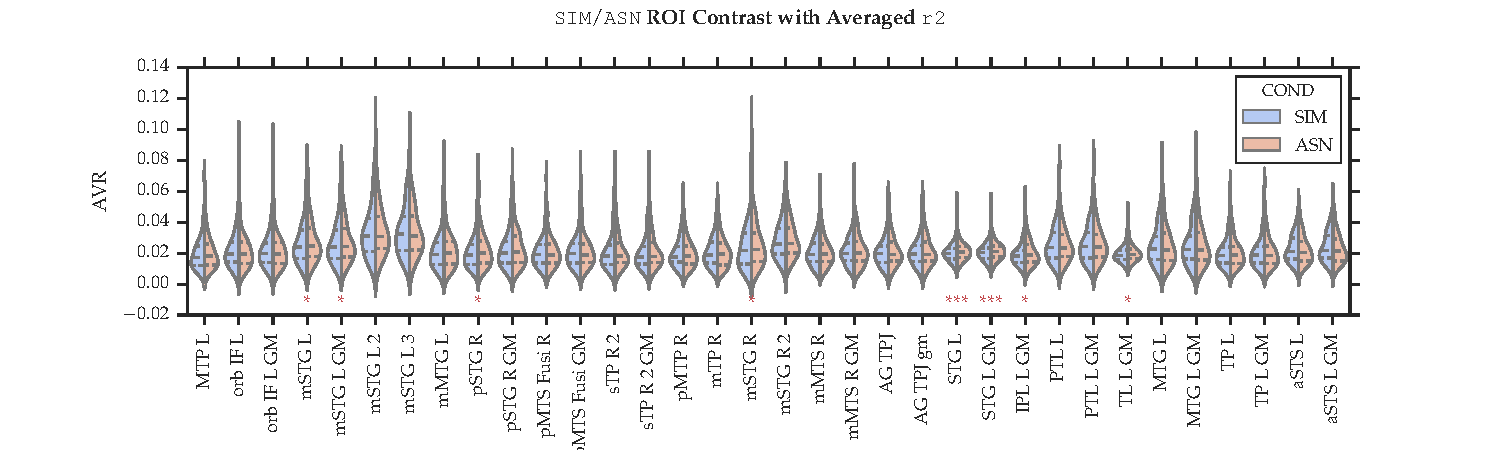
\includegraphics[width=\paperwidth]{Figures/SIM_ASN_ROI.pdf}
    }
    \caption[\code{SIM}-\code{ASN} ROI Contrast, Group]{*: p<0.05 uncorrected, ***: 0.05 ROI-wise multi-comparison corrected. Red color for \code{ASN}.\\ The average \code{r2} of voxels in a ROI is computed. We select only ROIs with scores>0.02 in either of \code{SIM} and \code{ASN} models. ROIs are of minimum size of 26 voxels (radius of 7 mm). None of the tested ROI reveals a significant mean difference in preference for \code{SIM}. ROIs in left middle-posterior STG, left inferior parietal lobe and left temporal lobe respond better to \code{ASN} model.} 
    \label{fig:SIM_ASN_ROI}
\end{figure}

\subsubsection{With \code{SIG}}

In general \code{SIG} [TODO]
